\section{Usage}
\label{sec:usage}

In this Section we show how to use PyDES (Pythonic Discrete Event Simulation), that is the software implemented to conduct all the experiments shown in this paper.

PyDES is a toolbox providing the user with commands to run simulations for the target system and randomness experiments on a Lehmer pseudo-random number generator.
The software comes with a handy CLI, providing the user with commands shown in Figure~\ref{fig:usage-cli-menu}. 

Every command implements an experiment generating both a textual reports, as the one shown in Figure~\ref{fig:usage-randomness-kolmogorov-smirnov}, and raw datasets that can be analyzed with the dedicated MATLAB live script, shown in Figure~\ref{fig:usage-matlab-live-script}. 
Commands running experiments with the simulator require longer configurations, hence they accept YAML configuration files, as the one shown in Figure~\ref{fig:usage-simulation-configuration}.

\begin{figure}
	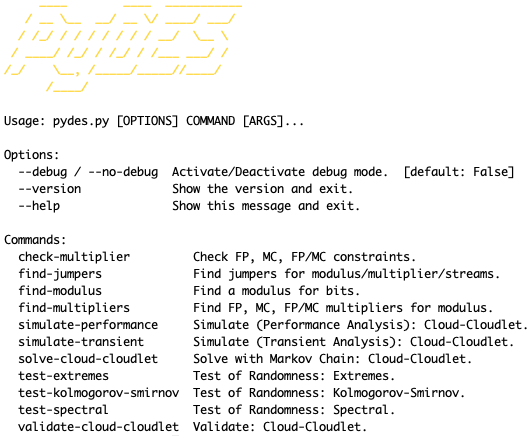
\includegraphics[width=\columnwidth]{fig/usage-pydes-cli}
	\caption{PyDES Command Line Interface.}
	\label{fig:usage-cli-menu}
\end{figure}

\begin{figure}
	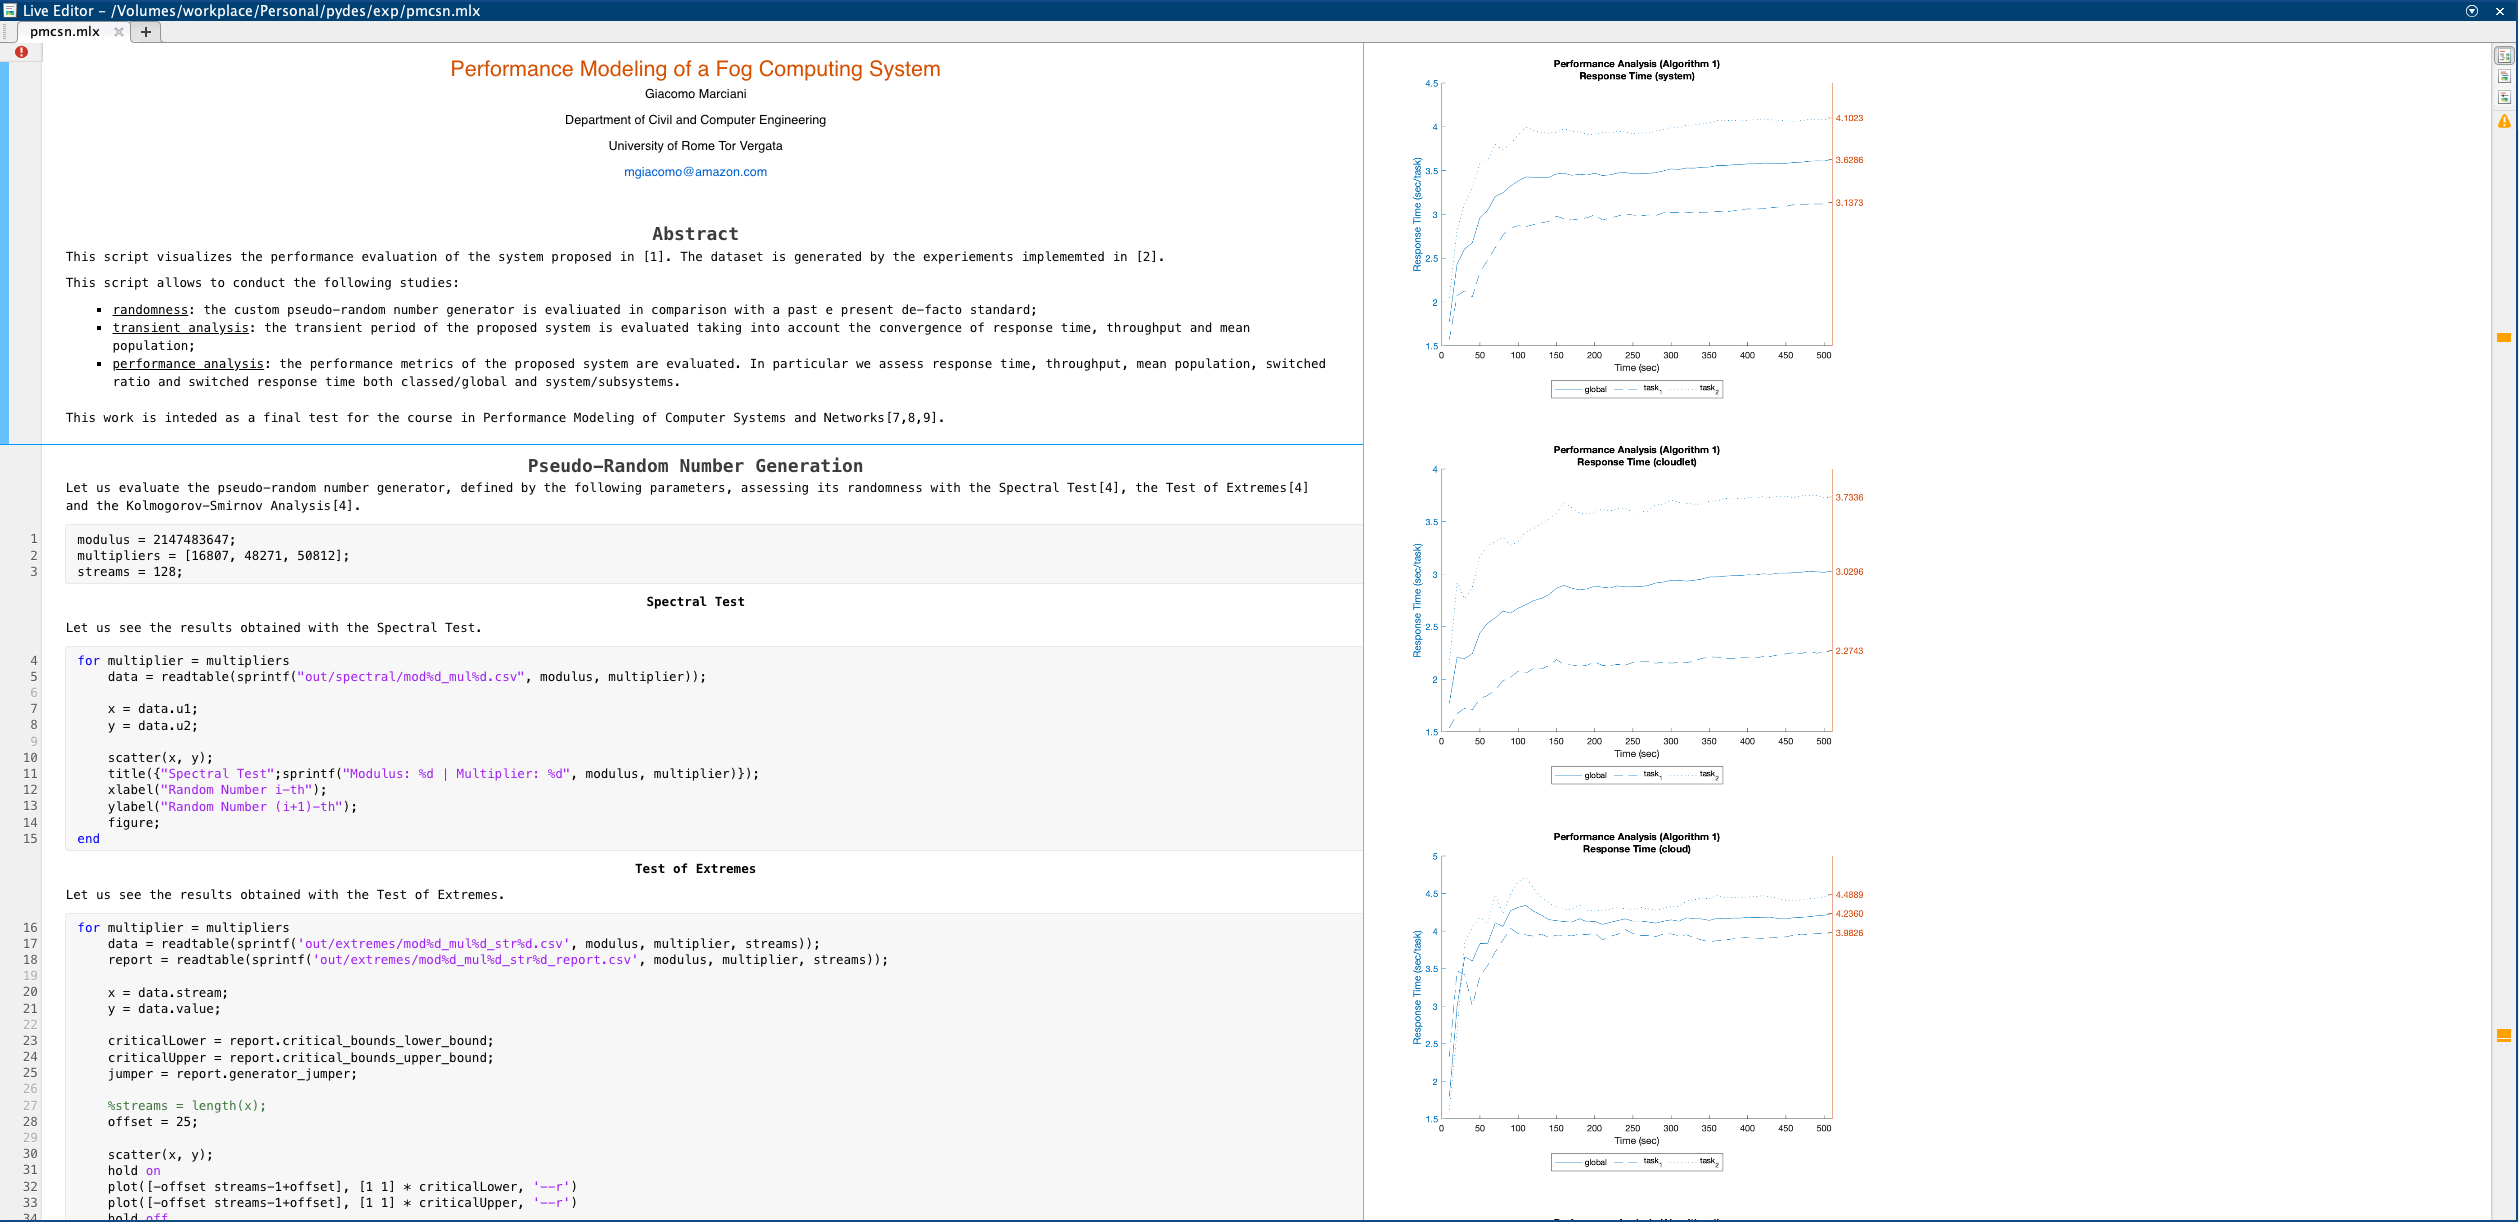
\includegraphics[width=\columnwidth]{fig/usage-matlab-live-script}
	\caption{MATLAB Live Script to visualize results.}
	\label{fig:usage-matlab-live-script}
\end{figure}

\begin{figure}
	\centering
	\lstinputlisting[basicstyle=\tiny]{ext/simulation-configuration-performance-analysis-2.yaml}
	\caption{Example: configuration for a simulation experiment.}
	\label{fig:usage-simulation-configuration}
\end{figure}

\begin{figure}
	\centering
	\lstinputlisting[basicstyle=\tiny]{ext/randomness-kolmogorov-smirnov.txt}
	\caption{Example: output report for a randomness experiment.}
	\label{fig:usage-randomness-kolmogorov-smirnov}
\end{figure}

\subsection{Simulation}
PyDES provides the user with the following commands to run simulation experiments:

\begin{itemize}
	
	\item \textbf{simulate-performance:} runs a simulation of the target system computing performance indices for the steady state leveraging the batch means method.
	\begin{lstlisting}[basicstyle=\tiny]
		pydes.py simulate-performance
		--config PATH
		--parameters JSON
	\end{lstlisting}
	
	\item \textbf{simulate-transient:} runs a simulation of the target system computing performance indices for the transient period. 
	\begin{lstlisting}[basicstyle=\tiny]
		pydes.py simulate-transient
		--config PATH
		--parameters JSON
	\end{lstlisting}
	
	\item \textbf{solve-cloud-cloudlet:} solves the target system using the analytical model shown in Section~\ref{sec:analytical-model}.
	\begin{lstlisting}[basicstyle=\tiny]
		pydes.py solve-cloud-cloudlet
		--config PATH
		--parameters JSON
	\end{lstlisting}
	
	\item \textbf{validate-cloud-cloudlet:} compares the experimental results obtained by the simulator with the ones obtained by the analytical model. In particular, it verifies for every performance index whether or not the analytical value belongs to the confidence interval determined by the simulator.
	\begin{lstlisting}[basicstyle=\tiny]
		pydes.py validate-cloud-cloudlet
		--analytical-result PATH
		--simulation-result PATH
	\end{lstlisting}
\end{itemize}

\subsection{Randomness}
PyDES provides the user with the following commands to run randomness experiments:

\begin{itemize}
	\item \textbf{check-multiplier:} checks the Full-Period (FP) and Modulus-Compatible (MC) constraints for a given modulus and multiplier.
	\begin{lstlisting}[basicstyle=\tiny]
pydes.py check-multiplier 
  --modulus INTEGER 
  --multiplier INTEGER
	\end{lstlisting}
	
	\item \textbf{find-jumpers:} determines a set of jumpers for a given modulus, multiplier and number of streams.
	\begin{lstlisting}[basicstyle=\tiny]
pydes.py find-jumpers
  --modulus INTEGER 
  --multiplier INTEGER
  --streams INTEGER
	\end{lstlisting}
	
	\item \textbf{find-modulus:} determines a modulus for a given number of bits.
	\begin{lstlisting}[basicstyle=\tiny]
pydes.py find-modulus
  --bits INTEGER
	\end{lstlisting}
	
	\item \textbf{find-multipliers:} determines a set of Full-Period/Modulus-Compatible multipliers for a given modulus.
	\begin{lstlisting}[basicstyle=\tiny]
pydes.py find-multipliers
  --modulus INTEGER
	\end{lstlisting}
	
	\item \textbf{test-extremes:} executes a Test of Extremes \cite{leemis2006discrete} on the given pseudo-random number generator. The output of this test is shown in Figure~\ref{fig:evaluation-randomness-extremes-50812}.
	\begin{lstlisting}[basicstyle=\tiny]
pydes.py test-extremes
  --modulus INTEGER
  --multiplier INTEGER
  --jumper INTEGER
  --streams INTEGER
  --samsize INTEGER 
  --bins INTEGER 
  --confidence FLOAT
  --d INTEGER
	\end{lstlisting}

	\item \textbf{test-kolmogorov-smirnov:} executes a Kolmogorov-Smirnov Test \cite{leemis2006discrete} on the given pseudo-random number generator. The current release only supports the Test of Extremes as the underlying Chi-square test. The output of this test is shown in Figure~\ref{fig:evaluation-randomness-kolmogorov-smirnov-50812}.
	
	\begin{lstlisting}[basicstyle=\tiny]
pydes.py test-kolmogorov-smirnov
  --modulus INTEGER
  --multiplier INTEGER
  --jumper INTEGER
  --streams INTEGER
  --test [extremes]
  --test-params JSON
	\end{lstlisting}
	
	\item \textbf{test-spectral:} executes a Spectral Test \cite{leemis2006discrete} on the given pseudo-random number generator, using it to generate a sample with the specified size and interval of values. The output of this test is shown in Figure~\ref{fig:evaluation-randomness-spectral-50812}.
	\begin{lstlisting}[basicstyle=\tiny]
pydes.py test-spectral
  --modulus INTEGER
  --multiplier INTEGER
  --samsize INTEGER
  --interval TUPLE
	\end{lstlisting}
	
\end{itemize}

